\section{ERNIE 1.0} \label{sec:ERNIE_1}

\subsection{Motivation for ERNIE 1.0}

Previous models like \nameref{sec:Word2Vec}, \nameref{sec:Glove}, and \nameref{sec:BERT} create word vector representations only through surrounding contexts, not also through prior knowledge in the sentence, and thus fail to capture relations between entities in a sentence. Consider the following training sentence: 

{\large \textit{``Harry Potter is a series of fantasy novels written by J. K. Rowling."}}

Using co-occurring words ``J.", ``K.", and ``Rowling", BERT can is limited to predicting the token ``K." but utterly fails at recognizing the whole entity \emph{J. K. Rowling}. A model could use simple co-occurrence counts to predict the missing entity \emph{Harry Potter} even without using long contexts, but it would not be making use of the relationship between the novel name and its writer. 

Current NLP models analyzing simple word co-occurrence may miss additional information like sentence order and nearness and named entities. 



This is where \textbf{ERNIE} steps in. \textbf{ERNIE (Enhanced Representation through Knowledge Integration)} can extrapolate the relationship between the \emph{Harry Potter} entity and \emph{J. K. Rowling} entity using implicit knowledge of words and entities, and uses this relationship to predict that Harry Potter is a series written by J. K. Rowling (Sun et al., 2019a). 



%\begin{figure}[h]
%\vspace{-5pt}
%\centering
%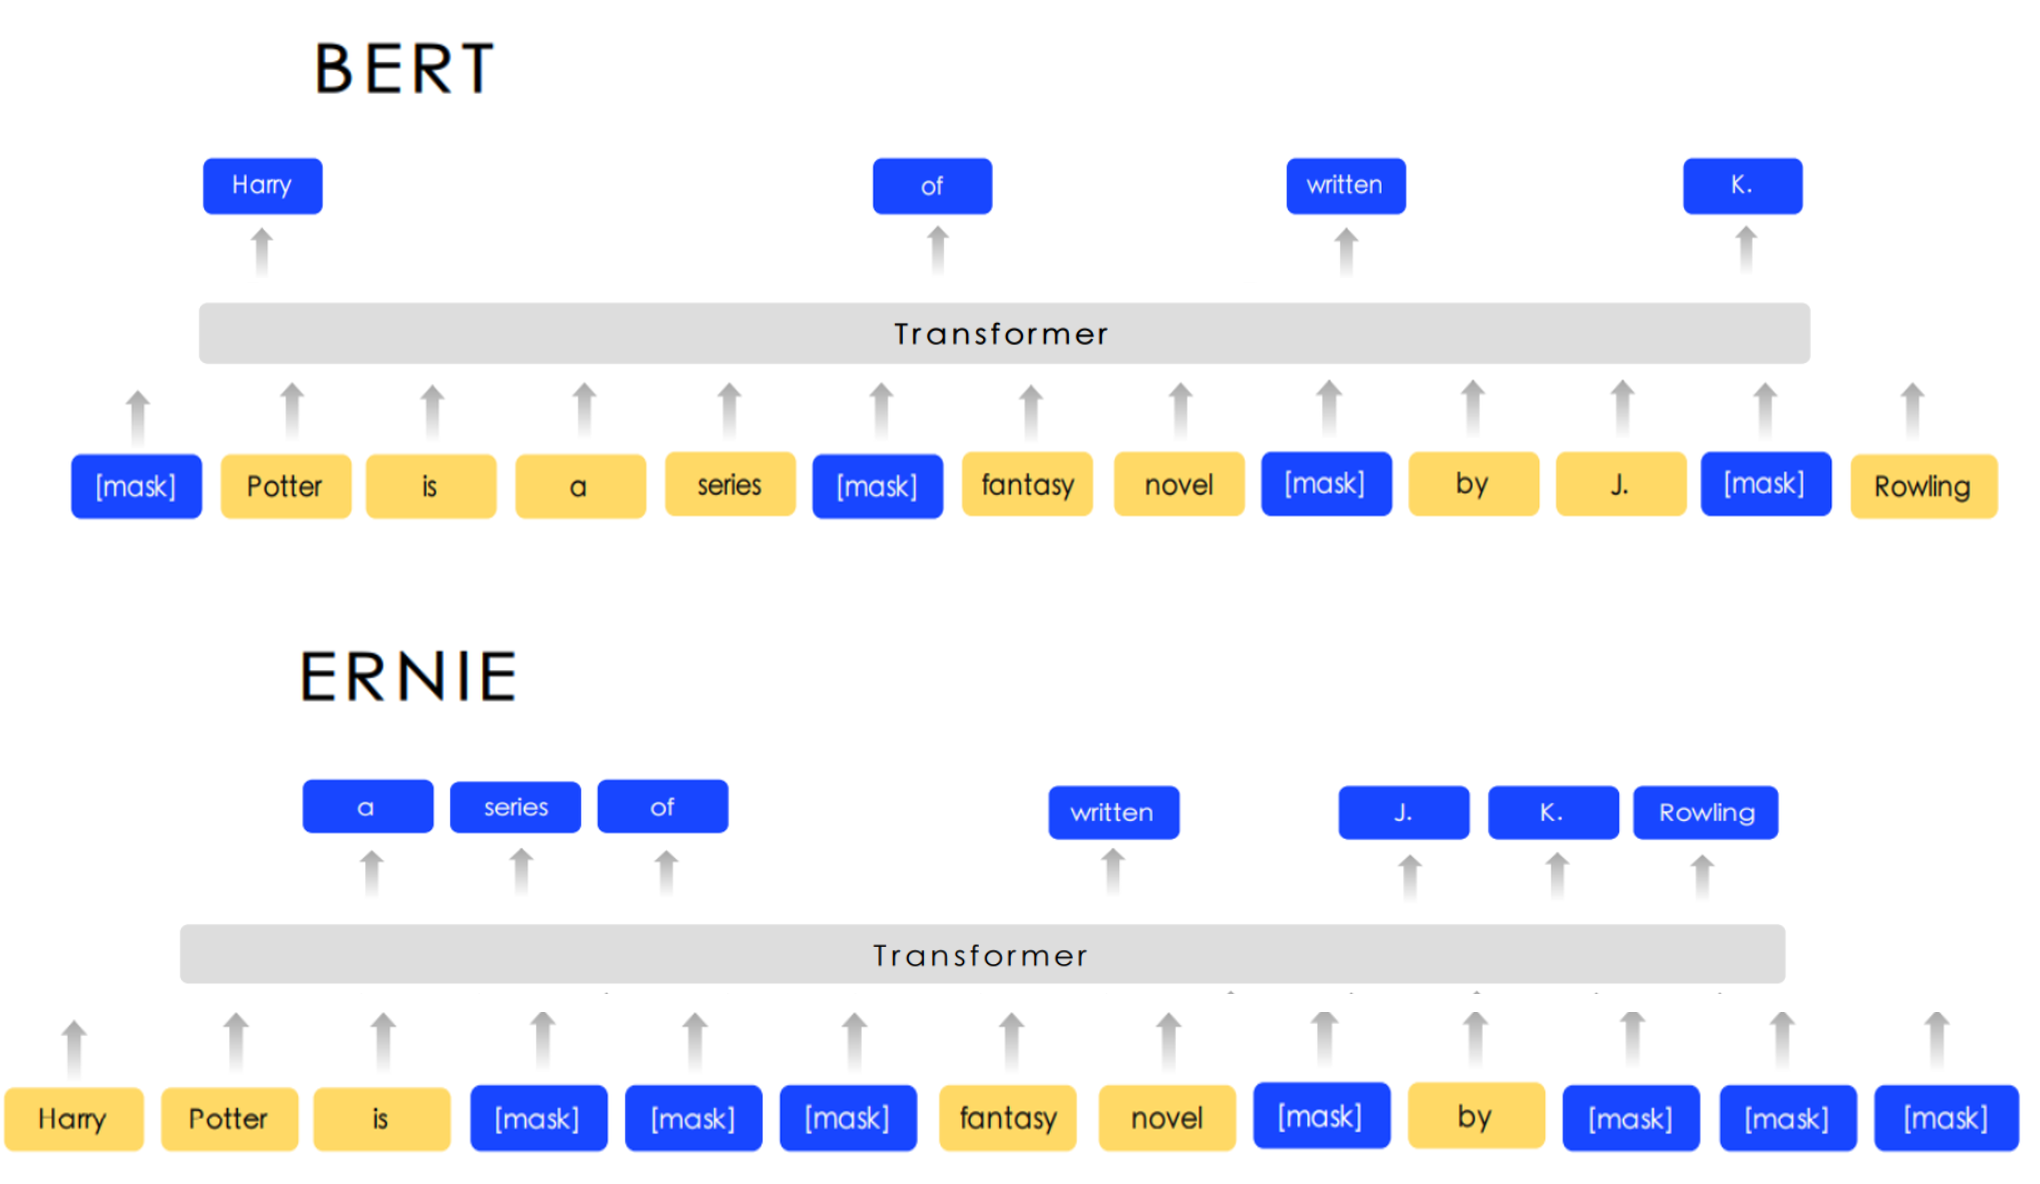
\includegraphics[width=0.9\textwidth]{imgs/ernie_vs_bert_masking.png}
%\vspace{-5pt}
%\captionof{figure}{\footnotesize Conceptual difference between \nameref{sec:BERT}'s masking and ERNIE's masking. From \emph{ERNIE: Enhanced Representation Through Knowledge Integration}, by Sun et al., 2019a. \url{https://arxiv.org/pdf/1904.09223.pdf}. Copyright 2019a by Sun et al.}
%\vspace{-5pt}
%\label{fig:ernie_vs_bert_masking}
%\end{figure}


ERNIE leverages a \nameref{sec:Transformer} encoder with \hyperref[sec:SelfAttention]{self-attention} alongside novel knowledge integration techniques like \nameref{sec:entitymasking} and \nameref{sec:phrasemasking} so that prior knowledge contained in conceptual units like phrases and entities can contribute to learning longer semantic dependencies for better model generalization and adaptability (Sun et al., 2019a). 


\subsubsection{phrase-level masking}\label{sec:phrasemasking}

A phrase is a ``small group of words of characters together acting as a conceptual unit" (Sun et al., 2019a). ERNIE uses lexical and chunking methods to determine phrase boundaries in sentences. In phrase-level masking, ERNIE randomly selects phrases from the sentences and masks them (as in \cref{fig:ernie_maskingTypes}), so that it can train by predicting the subpieces of the phrase. This way, phrase information can be built into ERNIE's learned word embeddings. 



\begin{figure}[h]
\vspace{-5pt}
\centering
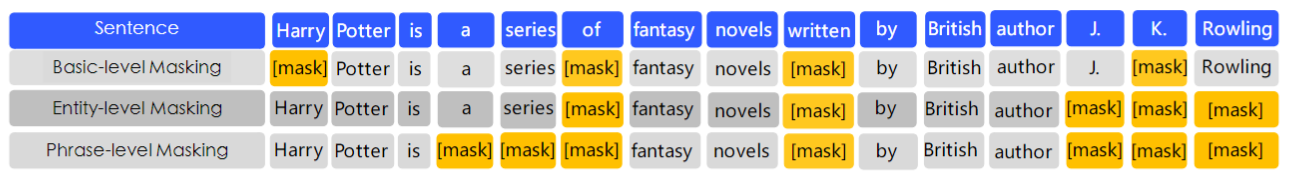
\includegraphics[width=0.99\textwidth]{imgs/ernie_maskingtypes.png}
\vspace{-5pt}
\captionof{figure}{\footnotesize ERNIE uses basic masking to get word representations, followed by phrase-level and entity-level masking. From \emph{ERNIE: Enhanced Representation Through Knowledge Integration}, by Sun et al., 2019. \url{https://arxiv.org/pdf/1904.09223.pdf}. Copyright 2019 by Sun et al.}
\vspace{-5pt}
\label{fig:ernie_maskingTypes}
\end{figure}


\subsubsection{entity-level masking}\label{sec:entitymasking}

Sun et al. (2019a) say that name entities contain ``persons, locations, organizations, products" which can be denoted with a proper name, and can be abstract or have physical existence. Entities often contain important information within a sentence, so are regarded as conceptual units. ERNIE parses a sentence for its named entities, then masks and predicts all slots within the entities, as shown in \cref{fig:ernie_maskingTypes}.


\subsection{Experimental Results of ERNIE 1.0}\label{sec:ExperimentalResultsERNIE}





% NOTE: the top width must be +0.5 more than below textwidth measure
\begin{program}
\begin{wrapfigure}{L}{0.6\textwidth}
\begin{center}
    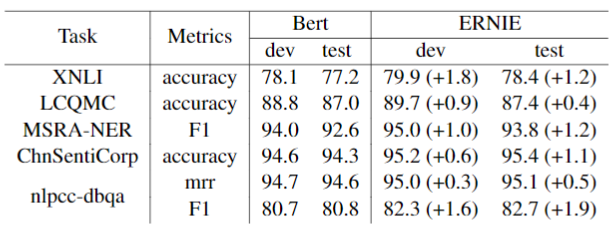
\includegraphics[width=0.55\textwidth]{imgs/ernie_tableResults.png}
\end{center}
\vspace{-20pt}
\captionof{table}{\footnotesize Comparing ERNIE and BERT on five major nlp tasks in Chinese. From \emph{Table 1 in ERNIE: Enhanced Representation Through Knowledge Integration}, by Sun et al., 2019. \url{https://arxiv.org/pdf/1904.09223.pdf}. Copyright 2019 by Sun et al.}
\vspace{-5pt}
\label{tbl:ernie_vs_bert_Results}
\end{wrapfigure}

As in \cref{tbl:ernie_vs_bert_Results}, ERNIE outperforms \nameref{sec:BERT} by more than $1 \%$ absolute accuracy on five Chinese NLP tasks: \nameref{nlptask:naturallanguageinferenceNLI} (XNLI data), \nameref{nlptask:semantictextualsimilaritySTS} (LCQMC data), \nameref{nlptask:namedentityrecognitionNER} (MSRA-NER data), \nameref{nlptask:sentimentanalysisSA} (ChnSentiCorp data), \nameref{nlptask:questionansweringQA} (NLPCC-DBQA data).

\end{program}



Sun et al. assert this is because of ERNIE's knowledge integration masking strategies, and this is supported in \cref{tbl:ernie_ablationStudy}; adding phrase masking to basic word-level masking improved ERNIE's performance almost a full percent, and adding entity-level masking to this combination resulted in still higher gains when sampling more data from larger texts. 


\begin{figure}[h]
\vspace{-5pt}
\centering
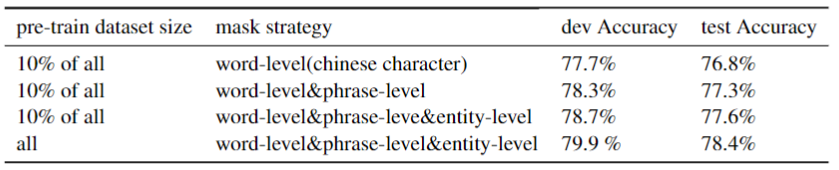
\includegraphics[width=0.8\textwidth]{imgs/ernie_tableAblation.png}
\vspace{-5pt}
\captionof{table}{\footnotesize Ablation study for ERNIE's \nameref{sec:phrasemasking} and \nameref{sec:entitymasking}. From \emph{Table 2 in ERNIE: Enhanced Representation Through Knowledge Integration}, by Sun et al., 2019. \url{https://arxiv.org/pdf/1904.09223.pdf}. Copyright 2019 by Sun et al.}
\vspace{-5pt}
\label{tbl:ernie_ablationStudy}
\end{figure}



Additionally, the authors tested ERNIE's knowledge learning ability using fill-in-the-blanks on named entities in paragraphs. In case 1 from \cref{tbl:ernie_vs_bert_knowledgeLearningTask}, ERNIE predicts the correct father name entity based on prior knowledge in the article while \nameref{sec:BERT} simply memorizes one of the sons' name, completely ignoring any relationship between mother and son. In case 2, \nameref{sec:BERT} can learn contextual patterns to predict the correct named entity type but fails to fill the slot with the actual correct entity, while ERNIE fills the slots with the correct entity. In cases 3,4,6 \nameref{sec:BERT} fills the slots with characters related to the sentences but not with the semantic concept, while ERNIE again predicts the correct entities. 


\begin{table}[htbp]
    \small 
    \centering
    \setlength{\tabcolsep}{6pt} % Default value: 6pt
    %\cellspacetoplimit = 6pt\cellspacebottomlimit =6pt
    \renewcommand{\arraystretch}{2} % Default value: 1
    
    \begin{tableFont}
    \begin{tabu} to \textwidth {| X[0.5] | X[7] | X | X | X |}
        
        \hline
      
        %\rowcolor{MyLavender} 
        \centering \textbf{Case}
        & \centering \textbf{Text} 
        & \centering \textbf{Predicted by ERNIE}\newline 
        & \centering\textbf{Predicted by BERT} 
        & \centering \textbf{Answer} \\ 
        
        \hline
        
        
        $1$
        &
        ``In September 2006, $\_\_\_$ married Cecilia Cheung. They had two sons, the older one is Zhenxuan Xie and the younger one is Zhennan Xie." \newline
        & 
        Tingfeng Xie
        & 
        Zhenxuan Xie
        & 
        {\color{Green} Tingfeng Xie} \\ 
        
        \hline 
        
        $2$
        &
        ``The Reform Movement of 1898, also known as the Hundred-Day Reform, was a bourgeois reform carried out by the reformists such as $\_\_\_$ and Qichao Liang through Emperor Guangxu."  \newline  
        & 
        Youwei Kang
        & 
        Schichang Sun
        & 
        {\color{Green} Youwei Kang} \\ 
        
        \hline 
        
        $3$
        &
        ``Hyperglycemia is caused by defective $\_\_\_$  secretion or impaired biological function, or both. Long-term hyperglycemia in diabetes leads to chronic damage and dysfunction of various tissues, generally eyes, kidneys, heart, blood vessels and nerves."   \newline 
        & 
        Insulin
        & 
        (Not a word in Chinese)
        & 
        {\color{Green} Insulin} \\ 
        
        \hline  
        
        $4$
        &
        ``Australia is a highly developed capitalist country with $\_\_\_$ as its capital. As the most developed country in the Southern Hemisphere, the $12$th largest economy in the world and the fourth largest exporter of agricultural products in the world, it is also the world's largest exporter of various minerals."   \newline 
        & 
        Melbourne
        & 
        (Not a city name)
        & 
        {\color{Green} Canberra} \\ 
        
        \hline 
        
        $6$
        &
        ``Relativity is a theory about space-time and gravity, which was founded by $\_\_\_$."   \newline 
        & 
        Einstein
        & 
        (Not a word in Chinese)
        & 
        {\color{Green} Einstein} \\ 
        
        
        \hline 
    \end{tabu}
    
    \end{tableFont}
    
    \captionof{table}{\footnotesize Comparing ERNIE to BERT on Cloze Chinese Task. From \emph{Figure 4 in ERNIE: Enhanced Representation Through Knowledge Integration}, by Sun et al., 2019. . Copyright 2019 by Sun et al.}
    
    \label{tbl:ernie_vs_bert_knowledgeLearningTask}
\end{table}




However in case 4, ERNIE predicts the wrong city name, though it still understands the semantic type. It is evident that ERNIE's contextual knowledge understanding is far superior to \nameref{sec:BERT}'s predictions (Sun et al., 2019a). 





% ------------------------------------------------------------

\section{ERNIE 2.0} \label{sec:ERNIE_2}


\subsection{Motivation for ERNIE 2.0}

Models such as \nameref{sec:Word2Vec}, \nameref{sec:Glove}, and \nameref{sec:BERT} extract meaning using co-occurrences. Even \nameref{sec:XLNet}'s permutation language model relies on co-occurrences. 


\begin{figure}[h]
\vspace{-5pt}
\centering
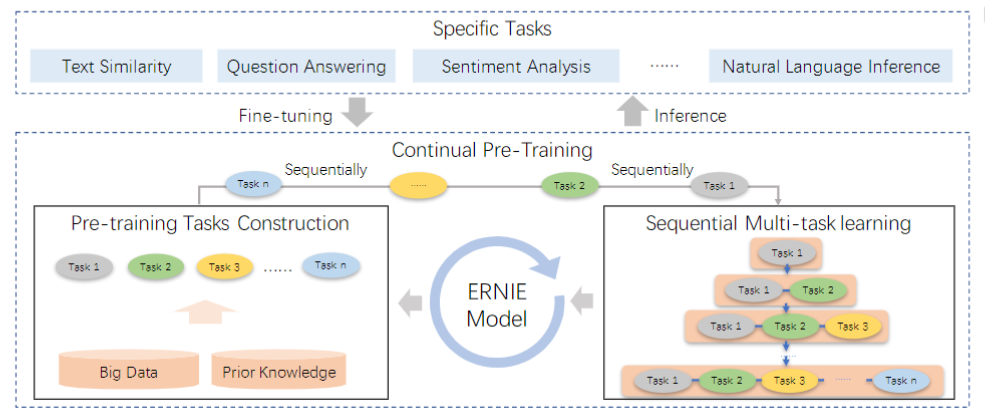
\includegraphics[width=0.9\textwidth]{imgs/ernie2_framework.png}
\vspace{-5pt}
\captionof{figure}{\footnotesize ERNIE 2.0's framework where embeddings are created by continual multi-task learning and then fine-tuned for specific \hyperref[app:Appendix_NLPTasks]{nlp tasks}. From \emph{Figure 1 in ERNIE 2.0: A Continual Pre-Training Framework for Language Understanding}, by Sun et al., 2019. \url{https://arxiv.org/pdf/1907.12412.pdf}. Copyright 2019 by Sun et al.}
\vspace{-5pt}
\label{fig:ernie2_framework}
\end{figure}


However, ERNIE 2.0 instead broadens the vision to more than just simple co-occurrence counts. Using a \hyperref[sec:ContinualMultiTaskLearning]{continual multi-task learning} framework (\cref{fig:ernie2_framework}) to remember previously learned knowledge, ERNIE 2.0 can capture ``lexical, syntactic and semantic information from training corpora in form of named entities (like person names,
location names, and organization names), semantic closeness (proximity of sentences),
sentence order or discourse relations” (Sun et al., 2019b).

\subsection{Continual Multi-Task Learning}\label{sec:ContinualMultiTaskLearning}

Traditional \textbf{continual learning} (Parisi et al. 2019; Chen and Liu, 2018) trains a model sequentially on multiple tasks to try to remember previously learned tasks while learning new ones. However, these procedures train the model with ``only one task at each stage with the demerit that it may forget previously learned knowledge" (Sun et al., 2019b). 





%%\begin{program}
%\begin{wrapfigure}{L}{0.7\textwidth}
%\begin{center}
%    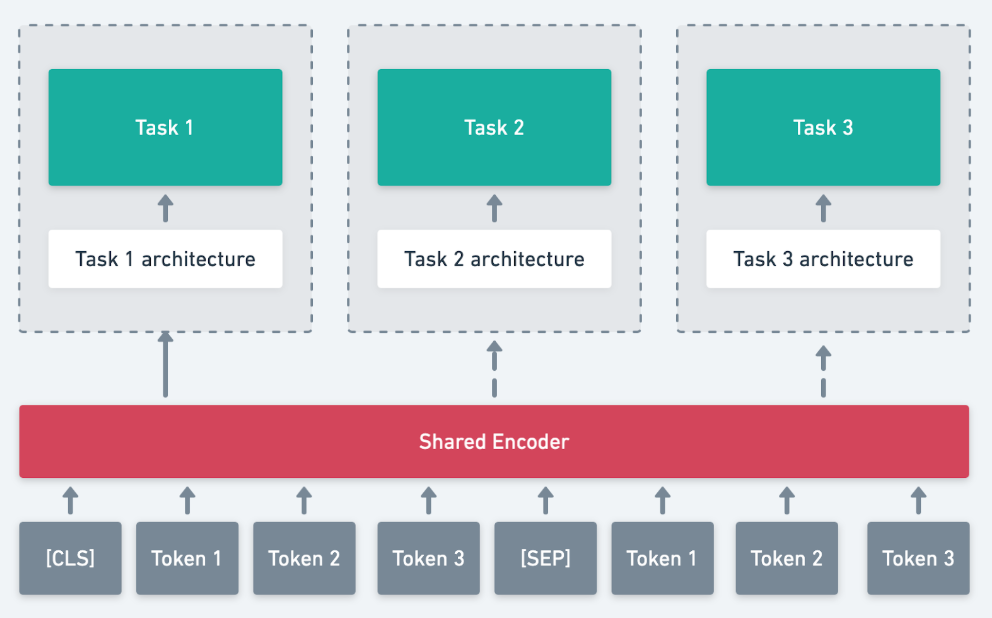
\includegraphics[width=0.6\textwidth]{imgs/multitaskExample.png}
%\end{center}
%%\vspace{-10pt}
%\captionof{figure}{\footnotesize Example of multi-task learning. From \emph{ERNIE 2.0: A Continual Pre-Training Framework for Language Understanding}, by Sequeira, 2019. \url{https://medium.com/psyai/ernie-2-0-an-article-to-hopefully-answer-all-your-questions-b5df21a64090}. Copyright n.d. by n.d.}
%%\vspace{-5pt}
%\label{fig:multitaskexample}
%\end{wrapfigure}

\textbf{Multi-task learning} means learning multiple tasks simultaneously. An Encoder is shared across task-specific architectures. In multitask model training, data is batched and allocated for specific task training. All tasks take turns learning on their mini-batched data then separately update the shared encoder based on the loss. However, this separate, individual task learning affects the weights in the shared encoder, causing ``catastrophic forgetting" (Sequeira, 2019). 

% An example is in \cref{fig:multitaskexample} where an Encoder is shared across task-specific architectures. 


%\end{program}




%\begin{program} % NOTE: program environment helps text start level with the wrapped figure, instead of filling up previous space. Was good for LSTM forget gates but here better without it. 



%\begin{wrapfigure}{L}{0.7\textwidth}
%    \begin{center}
%        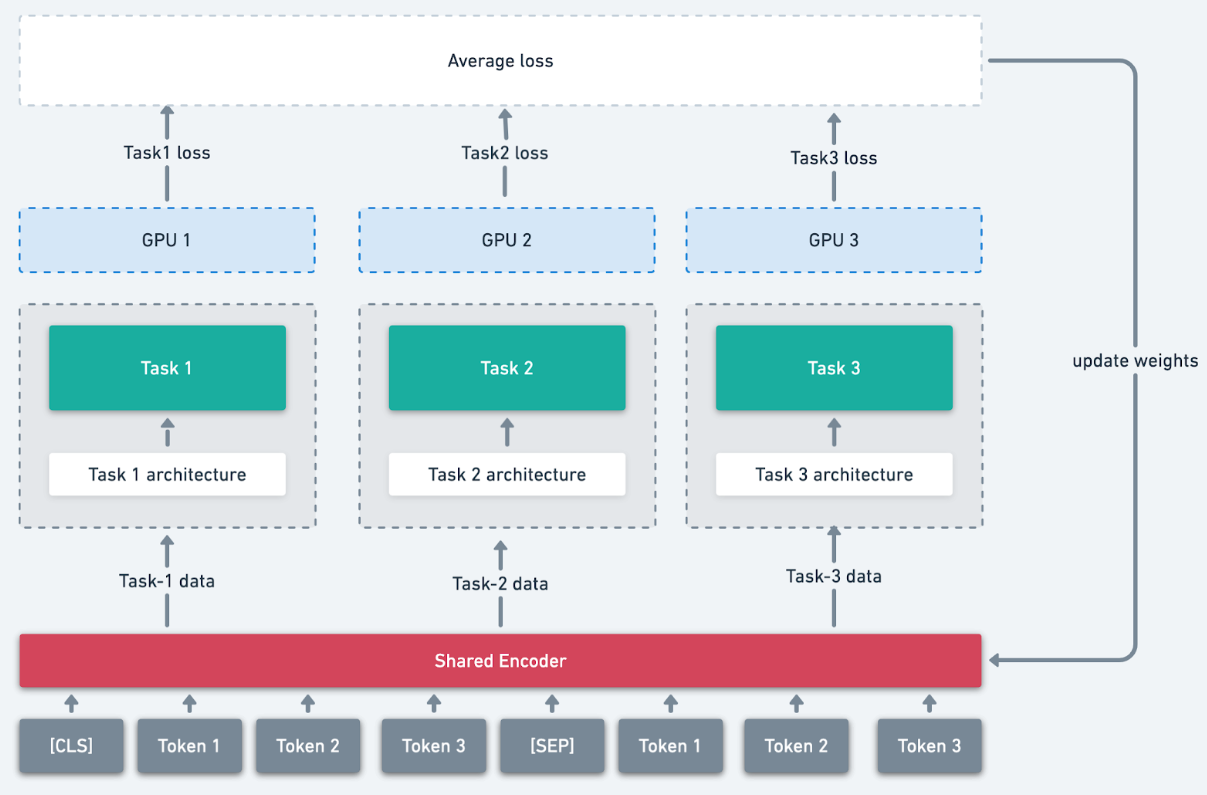
\includegraphics[width=0.65\textwidth]{imgs/ernie_continualMultitask.png}
%    \end{center}
%\vspace{-5pt}
%\captionof{figure}{\footnotesize Continual multi-task framework in ERNIE 2.0, where encoder can be a \hyperref[sec:RNN]{recurrent neural network (RNN)} or \nameref{sec:Transformer}. From \emph{ERNIE 2.0: A Continual Pre-Training Framework for Language Understanding}, by Sequeira, 2019. \url{https://medium.com/psyai/ernie-2-0-an-article-to-hopefully-answer-all-your-questions-b5df21a64090}. Copyright n.d. by n.d.}
%\vspace{-10pt}
%\label{fig:ernie_continualMultitaskLearning}
%\end{wrapfigure}

Inspired by human's ability to continuously accumulate information from past experience to develop new skills, \textbf{continual multi-task learning}  combines \textbf{continual learning} and \textbf{multi-task learning}. Humans do not forget skating when learning how to ski; continual multi-task learning helps a model do likewise. It trains several tasks in parallel and the shared encoder is updated using the average of losses from all tasks. Specifically, for the first step, only Task 1 is learned and the encoder weights are updated from Task 1's loss. In step 2, the shared encoder is initialized with weights from the previous step and Task 1 and 2 are learned at the same time. Since the shared encoder has already learned from Task 1, only the loss from Task 2 will mostly updated the shared encoder, while retaining Task 1 information. Next, average loss is calculated to update the shared encoder. These steps continue until the model has trained on all tasks (Sequeira, 2019). ERNIE has two kinds of loss functions: the token-level loss and the sentence-level loss. In this way, ERNIE is similar to the \nameref{sec:TransformerXL} which respects sentence structure. During pre-training, ERNIE combines the sentence-level loss function with multiple token-level loss functions to update the model continually (Sun et al., 2019b). 

%\end{program}




\subsection{Continual Pre-Training}\label{sec:ContinualPreTraining}

ERNIE 2.0's pre-training component differs from previous pre-training ones since rather than using few pre-training objectives, it continually interweaves a large variety of \hyperref[sec:WordAwarePretrainingTask]{word-aware}, \hyperref[sec:StructureAwarePretrainingTask]{structure-aware}, and \hyperref[sec:SemanticAwarePretrainingTask]{semantic-aware} pre-training tasks for capturing lexical, syntactic and semantic representations. The \textbf{continual pre-training} procedure has two steps: (1) continually create unsupervised pre-training tasks with large data and prior knowledge (like named entities, phrases, and discourse relations), and (2) use \hyperref[sec:ContinualMultiTaskLearning]{continual multi-task learning} to update ERNIE incrementally (Sun et al., 2019b). All the pre-training tasks are classification types and are described below. 

\subsubsection{Word-Aware Pre-Training Tasks}\label{sec:WordAwarePretrainingTask}

These tasks help ERNIE learn better representations at the word level. Closely following descriptions from Sun et al. (2019b): 

\begin{itemizeSpaced}{4pt}
    \item \textbf{Knowledge-Masking Task: }ERNIE masks words, phrases, and named entities then predicts them to learn dependency in local and global contexts. 
    
    \item \textbf{Capitalization Prediction Task: }to classify whether a word is capitalizated or not. The reason for this task is that capitalized words usually specific kinds of semantic information compared to latter words in a sentence. 
    
    \item \textbf{Token-Document Relation Prediction Task: } this task predicts if a token in a segment appears in other segments of the original document. The reason for this is that words appearing many times are common or relevant to the document's topic, and so can help the model capture the document's theme. 
    
\end{itemizeSpaced}



\subsubsection{Structure-Aware Pre-Training Tasks}\label{sec:StructureAwarePretrainingTask}

Structure-aware pre-training tasks help the model learn how sentences are related in a document. 

\begin{itemizeSpaced}{4pt}

    \item \textbf{Sentence Reordering Task: }a paragraph is broken into chunks, shuffled, and the model must reorder the shuffled segments into the original paragraph. 
    
    \item \textbf{Sentence Distance Task: }the model classifies if ``0" two sentences are adjacent in the same document, ``1" two sentences are in the same document but not adjacent, and ``2" two sentences are from two different documents.
\end{itemizeSpaced}



\subsubsection{Semantic-Aware Pre-Training Tasks}\label{sec:SemanticAwarePretrainingTask}

These tasks help ERNIE learn the semantics of sentences. 

\begin{itemizeSpaced}{4pt}

    \item \textbf{Discourse Relation Task: }to predict the semantic or rhetorical relation between two sentences. For example, ``The pine tree crashed to the ground. \textit{[because]} The strong mountain winds were merciless." The model must predict the discourse marker ``because", showing it learns the contrast between the two sentences, and in doing so, their semantics. 
    
    \item \textbf{Information Retrieval (IR) Relevance Task: }given a pair of user query and a document, the task is to classify if the document is strongly-relevant, weakly-relevant, or irrelevant or random to the user query, in terms of semantic information. This task helps ERNIE learn the semantics of the user query with respect to the document title. 
    
\end{itemizeSpaced}



\subsection{Experimental Results of ERNIE 2.0}\label{sec:ExperimentalResultsERNIE2}

In \cref{tbl:ernie2_bert_xlnet_expresults}, ERNIE 2.0 outperforms \nameref{sec:BERT} and even \nameref{sec:XLNet} for most of the English tasks, as measured by GLUE benchmark (Sun et al., 2019b). 

\begin{figure}[h]
\vspace{-5pt}
\centering
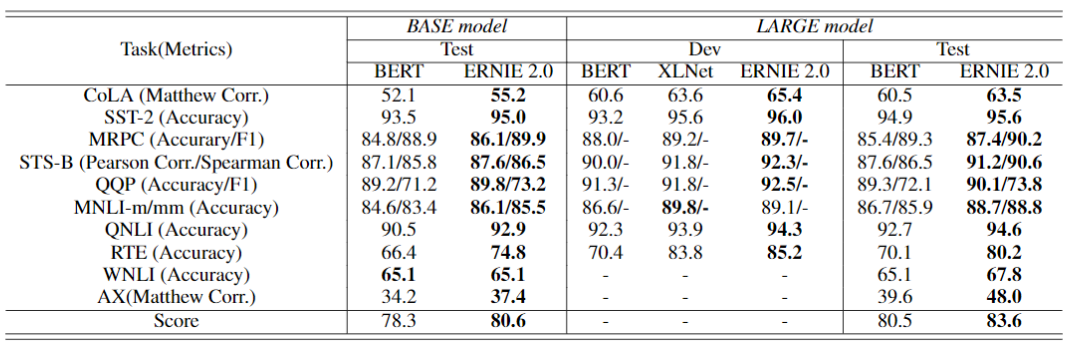
\includegraphics[width=0.9\textwidth]{imgs/ernie2_tableBERTvsERNIE2vsXLNET.png}
\vspace{-5pt}
\captionof{table}{\footnotesize Results on GLUE benchmark, where dev set contains medium of five runs and test set is scored by GLUE server. State of the art results are in bold. From \emph{Table 5 in ERNIE 2.0: A Continual Pre-Training Framework for Language Understanding}, by Sun et al., 2019. \url{https://arxiv.org/pdf/1907.12412.pdf}. Copyright 2019 by Sun et al.}
\vspace{-5pt}
\label{tbl:ernie2_bert_xlnet_expresults}
\end{figure}

The models \nameref{sec:BERT}, \nameref{sec:XLNet}, and \nameref{sec:ERNIE_2} were compared on Chinese tasks: machine reading comprehension (MRC) (CMRC dataset), \nameref{nlptask:namedentityrecognitionNER} (MSRA-NER dataset), \nameref{nlptask:naturallanguageinferenceNLI} (XNLI dataset), \nameref{nlptask:sentimentanalysisSA} (ChnSenitCorp dataset), \nameref{nlptask:semantictextualsimilaritySTS} (LCQMC dataset), and \nameref{nlptask:questionansweringQA} (NLPCC-DBQA dataset). \cref{tbl:ernie2_bert_xlnet_expresults} shows that \nameref{sec:ERNIE_1} outperforms \nameref{sec:BERT} in several tasks, but not all, while \nameref{sec:ERNIE_2} outperforms both previous models on all tasks (Sun et al., 2019b). 


\begin{figure}[h]
\vspace{-5pt}
\centering
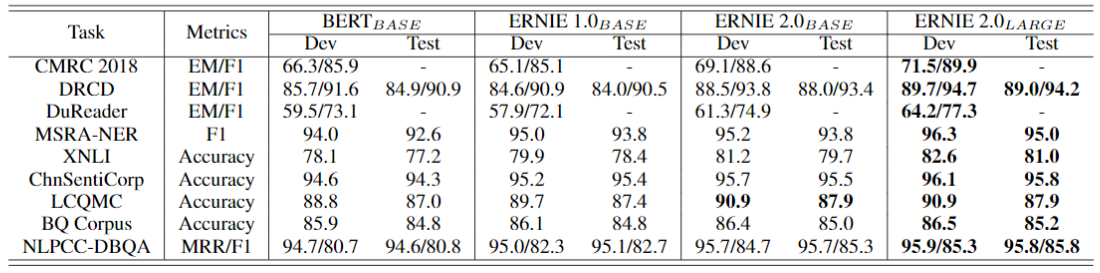
\includegraphics[width=0.9\textwidth]{imgs/ernie2_tableBERTvs_e2_e1.png}
\vspace{-5pt}
\captionof{table}{\footnotesize Results of Chinese \hyperref[app:Appendix_NLPTasks]{nlp tasks}. State of the art results are bolded. From \emph{Table 6 in ERNIE 2.0: A Continual Pre-Training Framework for Language Understanding}, by Sun et al., 2019. \url{https://arxiv.org/pdf/1907.12412.pdf}. Copyright 2019 by Sun et al.}
\vspace{-5pt}
\label{tbl:ernie2_ernie1_bert_expresults}
\end{figure}

In \cref{tbl:ernie2_comparePretrainings}, we see how multi-task learning trains all tasks simultaneously, continual learning trains the tasks one by one, while ERNIE 2.0's continual multi-task learning can allocate different iterations to each task in the various stages of training. Continual multi-task learning scores higher on the MNLI, SST-2, and MRPC datasets than the other two pre-training methods, confirming the guess that separately, multi-task and continual learning are prone to forgetting and other inefficiencies (Sun et al., 2019b). 

\begin{figure}[h]
\vspace{-5pt}
\centering
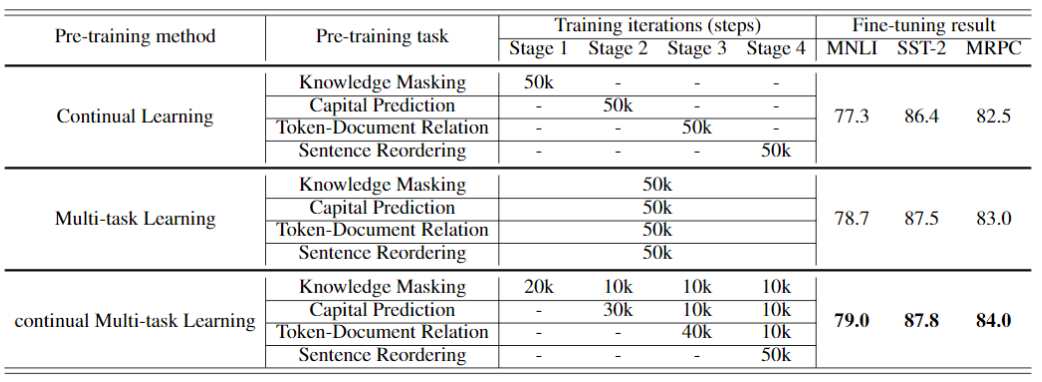
\includegraphics[width=0.9\textwidth]{imgs/ernie2_tableComparePretrainings.png}
\vspace{-5pt}
\captionof{table}{\footnotesize Experimental results of the different continual pre-training methods, using knowledge-masking, capital prediction, token-document, and sentence reording pre-training tasks. From \emph{Table 7 in ERNIE 2.0: A Continual Pre-Training Framework for Language Understanding}, by Sun et al., 2019. \url{https://arxiv.org/pdf/1907.12412.pdf}. Copyright 2019 by Sun et al.}
\vspace{-5pt}
\label{tbl:ernie2_comparePretrainings}
\end{figure}